\documentclass[twoside]{book}

% Packages required by doxygen
\usepackage{calc}
\usepackage{doxygen}
\usepackage{graphicx}
\usepackage[utf8]{inputenc}
\usepackage{makeidx}
\usepackage{multicol}
\usepackage{multirow}
\usepackage{fixltx2e}
\PassOptionsToPackage{warn}{textcomp}
\usepackage{textcomp}
\usepackage[nointegrals]{wasysym}
\usepackage[table]{xcolor}

% Font selection
\usepackage[T1]{fontenc}
\usepackage{mathptmx}
\usepackage[scaled=.90]{helvet}
\usepackage{courier}
\usepackage{amssymb}
\usepackage{sectsty}
\renewcommand{\familydefault}{\sfdefault}
\allsectionsfont{%
  \fontseries{bc}\selectfont%
  \color{darkgray}%
}
\renewcommand{\DoxyLabelFont}{%
  \fontseries{bc}\selectfont%
  \color{darkgray}%
}
\newcommand{\+}{\discretionary{\mbox{\scriptsize$\hookleftarrow$}}{}{}}

% Page & text layout
\usepackage{geometry}
\geometry{%
  a4paper,%
  top=2.5cm,%
  bottom=2.5cm,%
  left=2.5cm,%
  right=2.5cm%
}
\tolerance=750
\hfuzz=15pt
\hbadness=750
\setlength{\emergencystretch}{15pt}
\setlength{\parindent}{0cm}
\setlength{\parskip}{0.2cm}
\makeatletter
\renewcommand{\paragraph}{%
  \@startsection{paragraph}{4}{0ex}{-1.0ex}{1.0ex}{%
    \normalfont\normalsize\bfseries\SS@parafont%
  }%
}
\renewcommand{\subparagraph}{%
  \@startsection{subparagraph}{5}{0ex}{-1.0ex}{1.0ex}{%
    \normalfont\normalsize\bfseries\SS@subparafont%
  }%
}
\makeatother

% Headers & footers
\usepackage{fancyhdr}
\pagestyle{fancyplain}
\fancyhead[LE]{\fancyplain{}{\bfseries\thepage}}
\fancyhead[CE]{\fancyplain{}{}}
\fancyhead[RE]{\fancyplain{}{\bfseries\leftmark}}
\fancyhead[LO]{\fancyplain{}{\bfseries\rightmark}}
\fancyhead[CO]{\fancyplain{}{}}
\fancyhead[RO]{\fancyplain{}{\bfseries\thepage}}
\fancyfoot[LE]{\fancyplain{}{}}
\fancyfoot[CE]{\fancyplain{}{}}
\fancyfoot[RE]{\fancyplain{}{\bfseries\scriptsize Generated on Sun Apr 12 2015 23\+:15\+:28 for My Project by Doxygen }}
\fancyfoot[LO]{\fancyplain{}{\bfseries\scriptsize Generated on Sun Apr 12 2015 23\+:15\+:28 for My Project by Doxygen }}
\fancyfoot[CO]{\fancyplain{}{}}
\fancyfoot[RO]{\fancyplain{}{}}
\renewcommand{\footrulewidth}{0.4pt}
\renewcommand{\chaptermark}[1]{%
  \markboth{#1}{}%
}
\renewcommand{\sectionmark}[1]{%
  \markright{\thesection\ #1}%
}

% Indices & bibliography
\usepackage{natbib}
\usepackage[titles]{tocloft}
\setcounter{tocdepth}{3}
\setcounter{secnumdepth}{5}
\makeindex

% Hyperlinks (required, but should be loaded last)
\usepackage{ifpdf}
\ifpdf
  \usepackage[pdftex,pagebackref=true]{hyperref}
\else
  \usepackage[ps2pdf,pagebackref=true]{hyperref}
\fi
\hypersetup{%
  colorlinks=true,%
  linkcolor=blue,%
  citecolor=blue,%
  unicode%
}

% Custom commands
\newcommand{\clearemptydoublepage}{%
  \newpage{\pagestyle{empty}\cleardoublepage}%
}


%===== C O N T E N T S =====

\begin{document}

% Titlepage & ToC
\hypersetup{pageanchor=false,
             bookmarks=true,
             bookmarksnumbered=true,
             pdfencoding=unicode
            }
\pagenumbering{roman}
\begin{titlepage}
\vspace*{7cm}
\begin{center}%
{\Large My Project }\\
\vspace*{1cm}
{\large Generated by Doxygen 1.8.7}\\
\vspace*{0.5cm}
{\small Sun Apr 12 2015 23:15:28}\\
\end{center}
\end{titlepage}
\clearemptydoublepage
\tableofcontents
\clearemptydoublepage
\pagenumbering{arabic}
\hypersetup{pageanchor=true}

%--- Begin generated contents ---
\chapter{Hierarchical Index}
\section{Class Hierarchy}
This inheritance list is sorted roughly, but not completely, alphabetically\+:\begin{DoxyCompactList}
\item Q\+Dialog\begin{DoxyCompactList}
\item \contentsline{section}{C\+P\+U}{\pageref{class_c_p_u}}{}
\item \contentsline{section}{Memory}{\pageref{class_memory}}{}
\item \contentsline{section}{Sett}{\pageref{class_sett}}{}
\item \contentsline{section}{Usr}{\pageref{class_usr}}{}
\end{DoxyCompactList}
\item Q\+Main\+Window\begin{DoxyCompactList}
\item \contentsline{section}{Main\+Window}{\pageref{class_main_window}}{}
\end{DoxyCompactList}
\end{DoxyCompactList}

\chapter{Class Index}
\section{Data Structures}
Here are the data structures with brief descriptions\+:\begin{DoxyCompactList}
\item\contentsline{section}{\hyperlink{class_website_info}{Website\+Info} }{\pageref{class_website_info}}{}
\end{DoxyCompactList}

\chapter{Class Documentation}
\section{C\+P\+U Class Reference}
\label{class_c_p_u}\index{C\+P\+U@{C\+P\+U}}


Object window \char`\"{}\+Cpu\char`\"{}.  


Inheritance diagram for C\+P\+U\+:\begin{figure}[H]
\begin{center}
\leavevmode
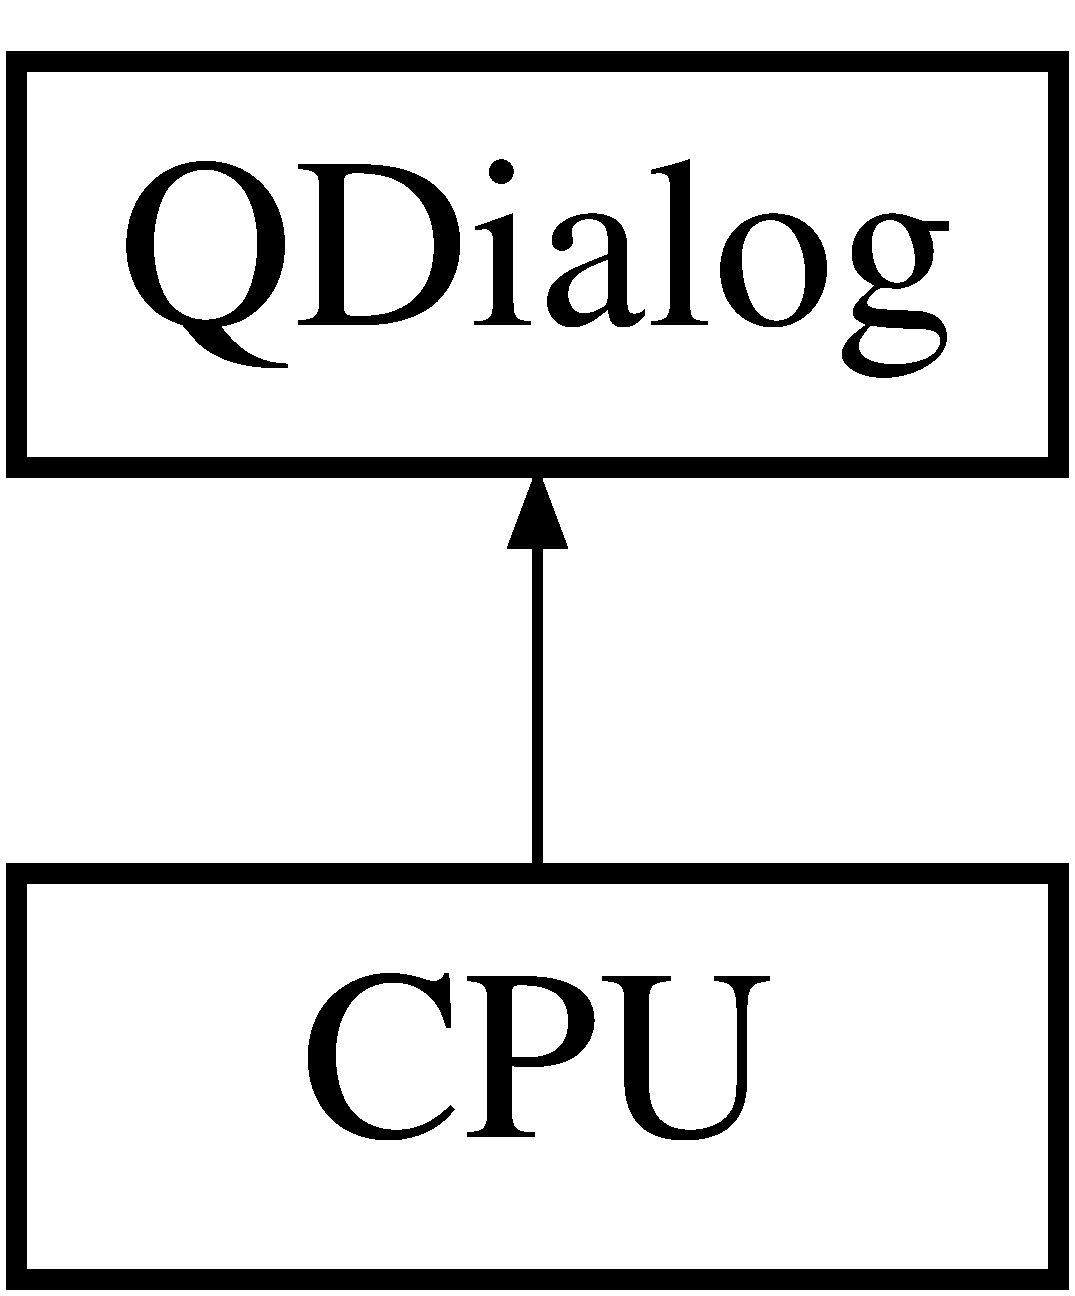
\includegraphics[height=2.000000cm]{class_c_p_u}
\end{center}
\end{figure}
\subsection*{Public Member Functions}
\begin{DoxyCompactItemize}
\item 
{\bf C\+P\+U} (Q\+Widget $\ast$parent=0)
\begin{DoxyCompactList}\small\item\em \doxyref{C\+P\+U\+::\+C\+P\+U}{p.}{class_c_p_u_a0155e9e9f7630a4114fbbfeb838c8e3f}. \end{DoxyCompactList}\item 
void {\bf center\+Window} ()
\begin{DoxyCompactList}\small\item\em It centers the widget on the screen. \end{DoxyCompactList}\end{DoxyCompactItemize}


\subsection{Detailed Description}
Object window \char`\"{}\+Cpu\char`\"{}. 

This class is meant to create an object window that shows the information of the \doxyref{C\+P\+U}{p.}{class_c_p_u} usage.

\begin{DoxyAuthor}{Author}
Camilla Lambrocco
\end{DoxyAuthor}
\begin{DoxyVersion}{Version}
1.\+1
\end{DoxyVersion}
\begin{DoxyDate}{Date}
4/12/2015 
\end{DoxyDate}


\subsection{Constructor \& Destructor Documentation}
\index{C\+P\+U@{C\+P\+U}!C\+P\+U@{C\+P\+U}}
\index{C\+P\+U@{C\+P\+U}!C\+P\+U@{C\+P\+U}}
\subsubsection[{C\+P\+U}]{\setlength{\rightskip}{0pt plus 5cm}C\+P\+U\+::\+C\+P\+U (
\begin{DoxyParamCaption}
\item[{Q\+Widget $\ast$}]{parent = {\ttfamily 0}}
\end{DoxyParamCaption}
)\hspace{0.3cm}{\ttfamily [explicit]}}\label{class_c_p_u_a0155e9e9f7630a4114fbbfeb838c8e3f}


\doxyref{C\+P\+U\+::\+C\+P\+U}{p.}{class_c_p_u_a0155e9e9f7630a4114fbbfeb838c8e3f}. 


\begin{DoxyParams}{Parameters}
{\em parent} & \\
\hline
\end{DoxyParams}


\subsection{Member Function Documentation}
\index{C\+P\+U@{C\+P\+U}!center\+Window@{center\+Window}}
\index{center\+Window@{center\+Window}!C\+P\+U@{C\+P\+U}}
\subsubsection[{center\+Window}]{\setlength{\rightskip}{0pt plus 5cm}void C\+P\+U\+::center\+Window (
\begin{DoxyParamCaption}
{}
\end{DoxyParamCaption}
)}\label{class_c_p_u_acd00910bff01f1314fc2cedd6cd61056}


It centers the widget on the screen. 

\begin{DoxyReturn}{Returns}
Void. 
\end{DoxyReturn}


The documentation for this class was generated from the following files\+:\begin{DoxyCompactItemize}
\item 
cpu.\+h\item 
cpu.\+cpp\end{DoxyCompactItemize}

\section{Main\+Window Class Reference}
\label{class_main_window}\index{Main\+Window@{Main\+Window}}


Object window \char`\"{}\+Main\char`\"{}.  


Inheritance diagram for Main\+Window\+:\begin{figure}[H]
\begin{center}
\leavevmode
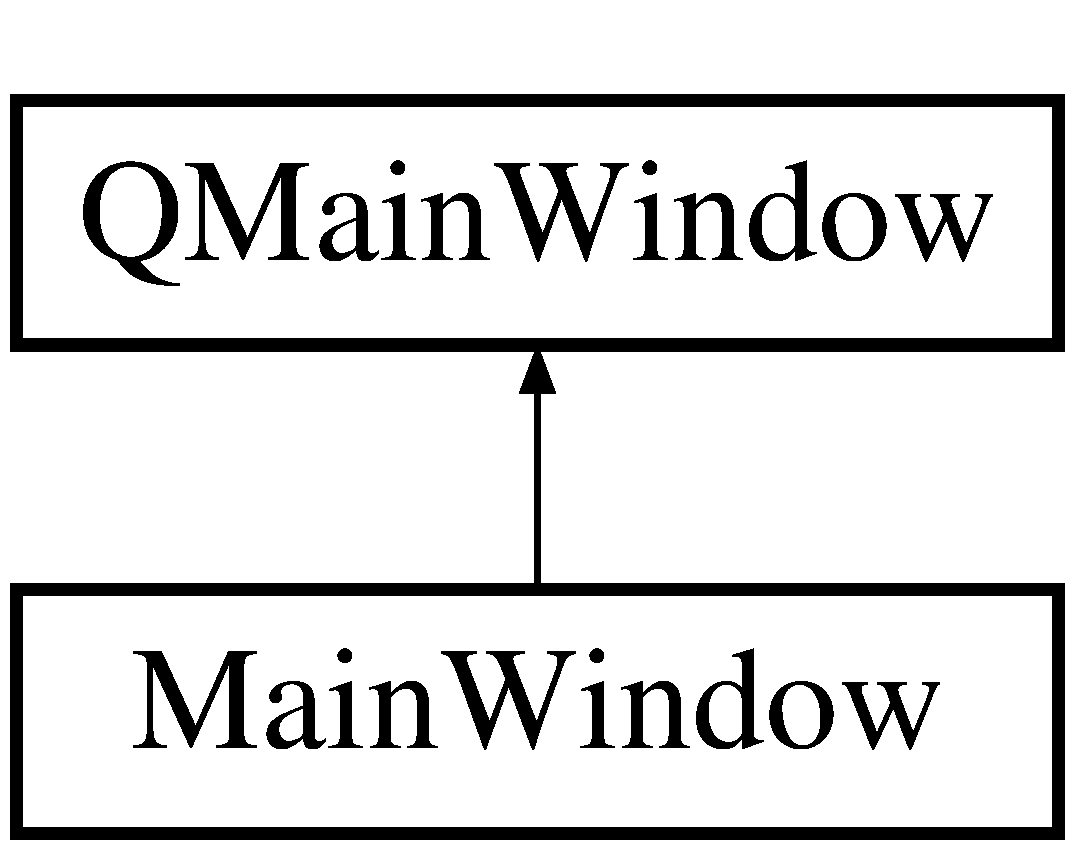
\includegraphics[height=2.000000cm]{class_main_window}
\end{center}
\end{figure}
\subsection*{Public Member Functions}
\begin{DoxyCompactItemize}
\item 
{\bf Main\+Window} (Q\+Widget $\ast$parent=0)
\begin{DoxyCompactList}\small\item\em \doxyref{Main\+Window\+::\+Main\+Window}{p.}{class_main_window_a8b244be8b7b7db1b08de2a2acb9409db}. \end{DoxyCompactList}\item 
void {\bf center\+Window} ()
\begin{DoxyCompactList}\small\item\em It centers the widget on the screen. \end{DoxyCompactList}\end{DoxyCompactItemize}


\subsection{Detailed Description}
Object window \char`\"{}\+Main\char`\"{}. 

This class is meant to create the main object window that shows date and time. It allows to pass to the \char`\"{}\+Settings\char`\"{} window or to quit the system.

\begin{DoxyNote}{Note}
Attempts at zen rarely work.
\end{DoxyNote}
\begin{DoxyAuthor}{Author}
Camilla Lambrocco
\end{DoxyAuthor}
\begin{DoxyVersion}{Version}
1.\+1
\end{DoxyVersion}
\begin{DoxyDate}{Date}
4/12/2015 
\end{DoxyDate}


\subsection{Constructor \& Destructor Documentation}
\index{Main\+Window@{Main\+Window}!Main\+Window@{Main\+Window}}
\index{Main\+Window@{Main\+Window}!Main\+Window@{Main\+Window}}
\subsubsection[{Main\+Window}]{\setlength{\rightskip}{0pt plus 5cm}Main\+Window\+::\+Main\+Window (
\begin{DoxyParamCaption}
\item[{Q\+Widget $\ast$}]{parent = {\ttfamily 0}}
\end{DoxyParamCaption}
)\hspace{0.3cm}{\ttfamily [explicit]}}\label{class_main_window_a8b244be8b7b7db1b08de2a2acb9409db}


\doxyref{Main\+Window\+::\+Main\+Window}{p.}{class_main_window_a8b244be8b7b7db1b08de2a2acb9409db}. 


\begin{DoxyParams}{Parameters}
{\em parent} & \\
\hline
\end{DoxyParams}


\subsection{Member Function Documentation}
\index{Main\+Window@{Main\+Window}!center\+Window@{center\+Window}}
\index{center\+Window@{center\+Window}!Main\+Window@{Main\+Window}}
\subsubsection[{center\+Window}]{\setlength{\rightskip}{0pt plus 5cm}void Main\+Window\+::center\+Window (
\begin{DoxyParamCaption}
{}
\end{DoxyParamCaption}
)}\label{class_main_window_a775d79cb8170d36faf4aa9ce4570d8b3}


It centers the widget on the screen. 

\begin{DoxyReturn}{Returns}
Void. 
\end{DoxyReturn}


The documentation for this class was generated from the following files\+:\begin{DoxyCompactItemize}
\item 
mainwindow.\+h\item 
mainwindow.\+cpp\end{DoxyCompactItemize}

\hypertarget{class_memory}{\section{Memory Class Reference}
\label{class_memory}\index{Memory@{Memory}}
}


Provide an example.  




{\ttfamily \#include $<$memory.\+h$>$}

Inheritance diagram for Memory\+:\begin{figure}[H]
\begin{center}
\leavevmode
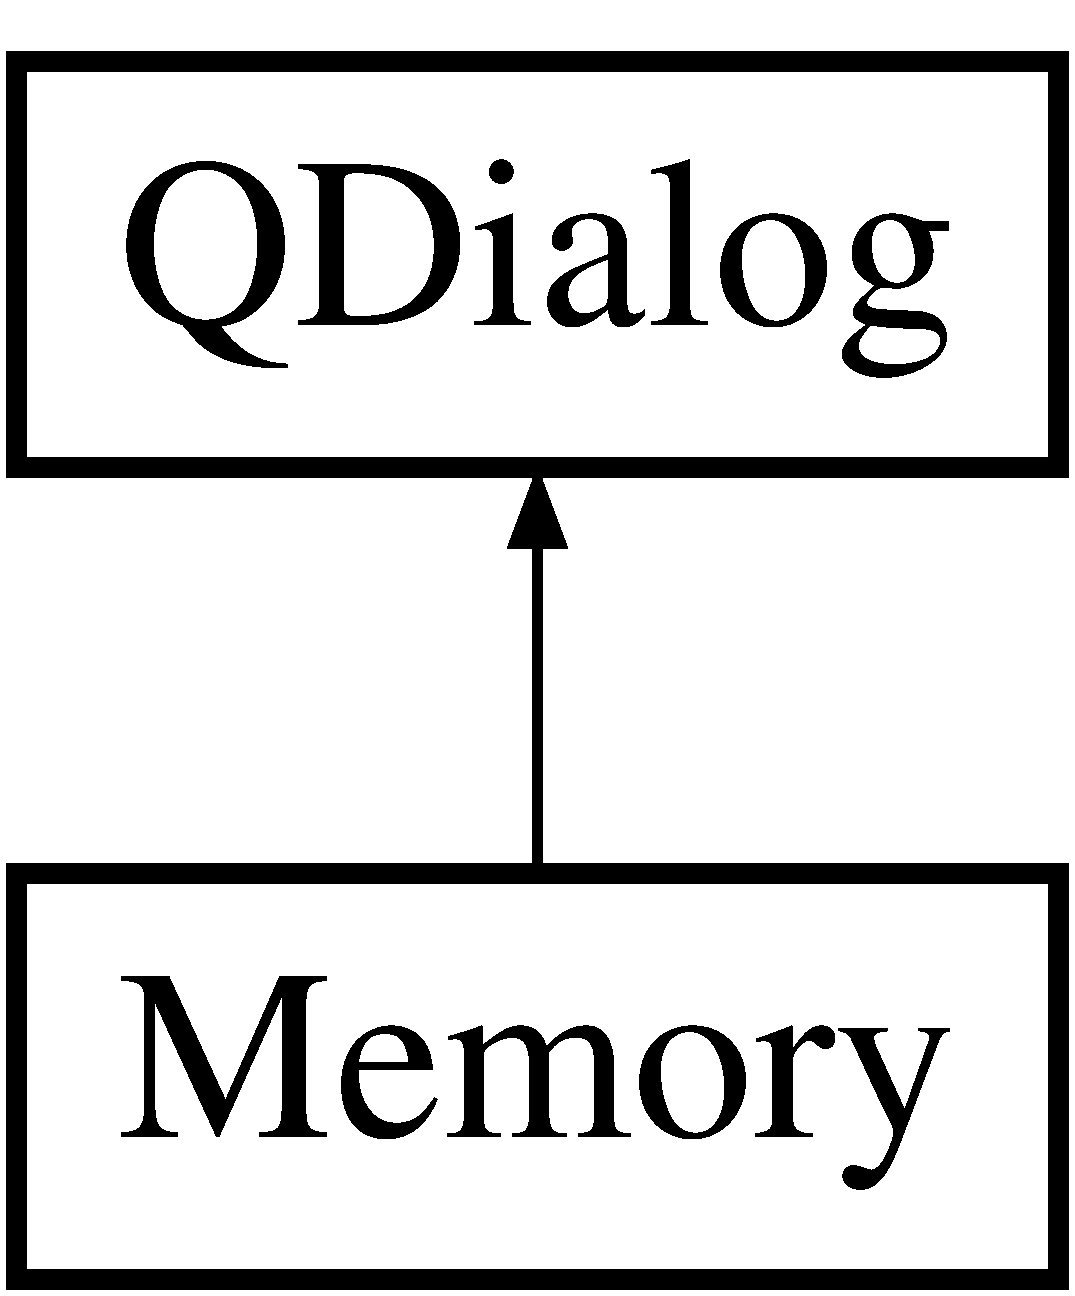
\includegraphics[height=2.000000cm]{class_memory}
\end{center}
\end{figure}
\subsection*{Public Member Functions}
\begin{DoxyCompactItemize}
\item 
\hyperlink{class_memory_a243eef3e0fd8d02131e3bcca0471c931}{Memory} (Q\+Widget $\ast$parent=0)
\begin{DoxyCompactList}\small\item\em \hyperlink{class_memory_a243eef3e0fd8d02131e3bcca0471c931}{Memory\+::\+Memory}. \end{DoxyCompactList}\item 
\hypertarget{class_memory_ac367017fbb51cb2d8a334b8063b0e7c2}{void {\bfseries update} ()}\label{class_memory_ac367017fbb51cb2d8a334b8063b0e7c2}

\item 
\hypertarget{class_memory_aedc640c354e83e9f415082bbed99a562}{void {\bfseries refresh} ()}\label{class_memory_aedc640c354e83e9f415082bbed99a562}

\item 
\hypertarget{class_memory_a365f73ddc2ac2c85241ecdbe6c61bf68}{void {\bfseries center\+Window} ()}\label{class_memory_a365f73ddc2ac2c85241ecdbe6c61bf68}

\end{DoxyCompactItemize}


\subsection{Detailed Description}
Provide an example. 

This class is meant as an example. It is not useful by itself rather its usefulness is only a function of how much it helps the reader. It is in a sense defined by the person who reads it and otherwise does not exist in any real form.

\begin{DoxyNote}{Note}
Attempts at zen rarely work.
\end{DoxyNote}
\begin{DoxyAuthor}{Author}

\end{DoxyAuthor}
\begin{DoxyParagraph}{Author}
Camilla Lambrocco 
\end{DoxyParagraph}


\begin{DoxyVersion}{Version}

\end{DoxyVersion}
\begin{DoxyParagraph}{Revision}
1.\+1 
\end{DoxyParagraph}


\begin{DoxyDate}{Date}

\end{DoxyDate}
\begin{DoxyParagraph}{Date}
4/12/2015 
\end{DoxyParagraph}


\subsection{Constructor \& Destructor Documentation}
\hypertarget{class_memory_a243eef3e0fd8d02131e3bcca0471c931}{\index{Memory@{Memory}!Memory@{Memory}}
\index{Memory@{Memory}!Memory@{Memory}}
\subsubsection[{Memory}]{\setlength{\rightskip}{0pt plus 5cm}Memory\+::\+Memory (
\begin{DoxyParamCaption}
\item[{Q\+Widget $\ast$}]{parent = {\ttfamily 0}}
\end{DoxyParamCaption}
)\hspace{0.3cm}{\ttfamily [explicit]}}}\label{class_memory_a243eef3e0fd8d02131e3bcca0471c931}


\hyperlink{class_memory_a243eef3e0fd8d02131e3bcca0471c931}{Memory\+::\+Memory}. 


\begin{DoxyParams}{Parameters}
{\em parent} & \\
\hline
\end{DoxyParams}


The documentation for this class was generated from the following files\+:\begin{DoxyCompactItemize}
\item 
memory.\+h\item 
memory.\+cpp\end{DoxyCompactItemize}

\hypertarget{class_sett}{\section{Sett Class Reference}
\label{class_sett}\index{Sett@{Sett}}
}


Provide an example.  




{\ttfamily \#include $<$sett.\+h$>$}

Inheritance diagram for Sett\+:\begin{figure}[H]
\begin{center}
\leavevmode
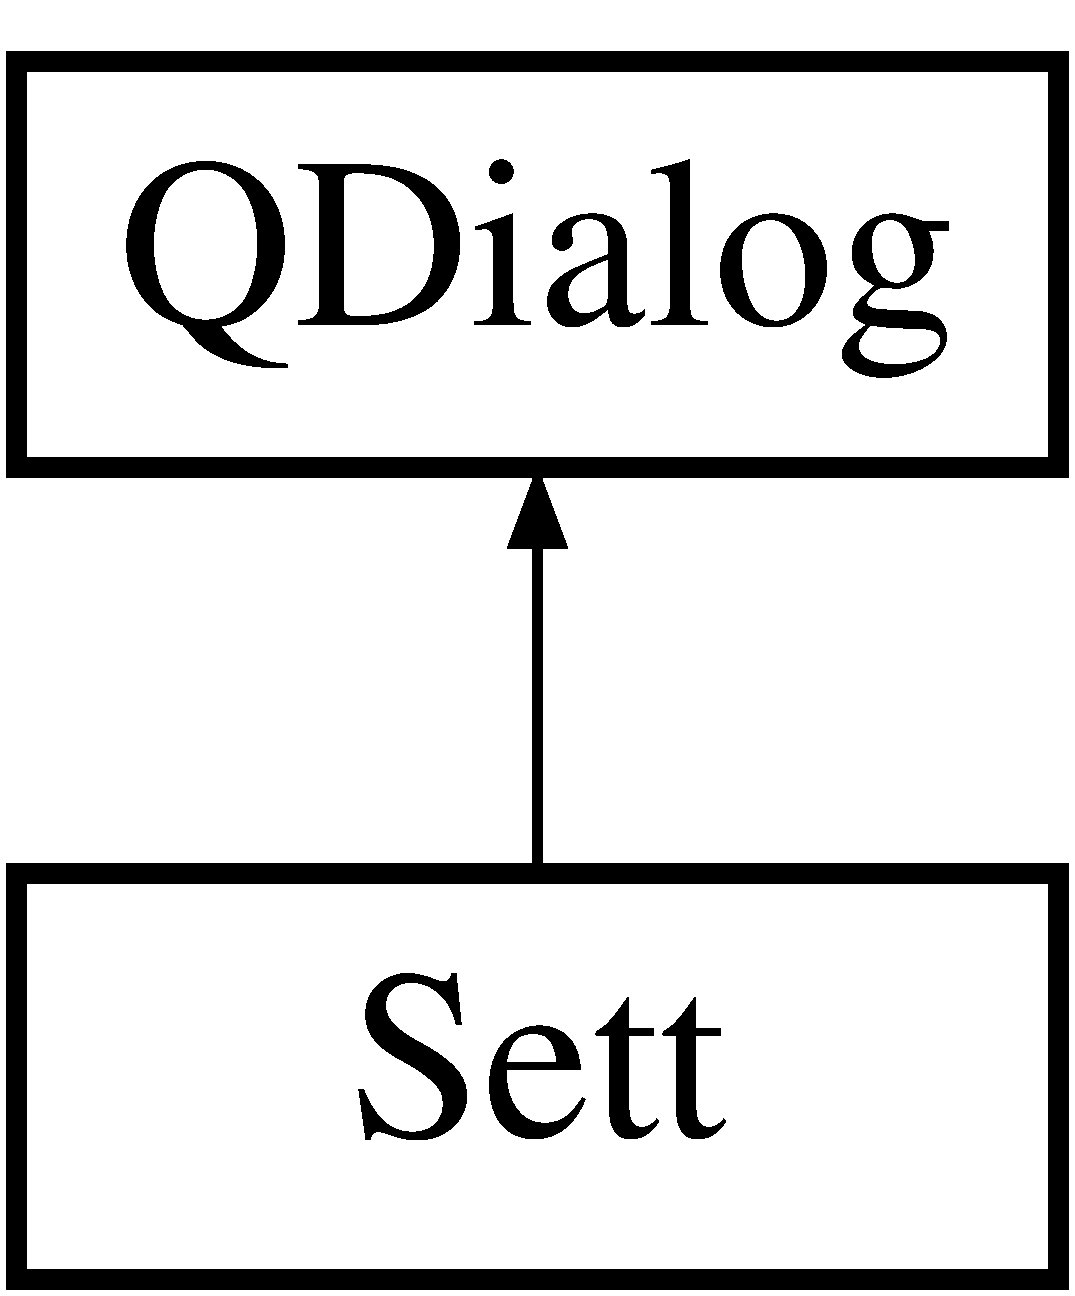
\includegraphics[height=2.000000cm]{class_sett}
\end{center}
\end{figure}
\subsection*{Public Member Functions}
\begin{DoxyCompactItemize}
\item 
\hyperlink{class_sett_abbc0a2f51e953575a6d456eee64a96de}{Sett} (Q\+Widget $\ast$parent=0)
\begin{DoxyCompactList}\small\item\em \hyperlink{class_sett_abbc0a2f51e953575a6d456eee64a96de}{Sett\+::\+Sett}. \end{DoxyCompactList}\item 
void \hyperlink{class_sett_a9e898b5c9359f7fb52910315d023283c}{center\+Window} ()
\begin{DoxyCompactList}\small\item\em Writes the current foreground and background color of characters printed on the console into the argument color. \end{DoxyCompactList}\end{DoxyCompactItemize}


\subsection{Detailed Description}
Provide an example. 

This class is meant as an example. It is not useful by itself rather its usefulness is only a function of how much it helps the reader. It is in a sense defined by the person who reads it and otherwise does not exist in any real form.

\begin{DoxyNote}{Note}
Attempts at zen rarely work.
\end{DoxyNote}
\begin{DoxyAuthor}{Author}

\end{DoxyAuthor}
\begin{DoxyParagraph}{Author}
Camilla Lambrocco 
\end{DoxyParagraph}


\begin{DoxyVersion}{Version}

\end{DoxyVersion}
\begin{DoxyParagraph}{Revision}
1.\+1 
\end{DoxyParagraph}


\begin{DoxyDate}{Date}

\end{DoxyDate}
\begin{DoxyParagraph}{Date}
4/12/2015 
\end{DoxyParagraph}


\subsection{Constructor \& Destructor Documentation}
\hypertarget{class_sett_abbc0a2f51e953575a6d456eee64a96de}{\index{Sett@{Sett}!Sett@{Sett}}
\index{Sett@{Sett}!Sett@{Sett}}
\subsubsection[{Sett}]{\setlength{\rightskip}{0pt plus 5cm}Sett\+::\+Sett (
\begin{DoxyParamCaption}
\item[{Q\+Widget $\ast$}]{parent = {\ttfamily 0}}
\end{DoxyParamCaption}
)\hspace{0.3cm}{\ttfamily [explicit]}}}\label{class_sett_abbc0a2f51e953575a6d456eee64a96de}


\hyperlink{class_sett_abbc0a2f51e953575a6d456eee64a96de}{Sett\+::\+Sett}. 


\begin{DoxyParams}{Parameters}
{\em parent} & \\
\hline
\end{DoxyParams}


\subsection{Member Function Documentation}
\hypertarget{class_sett_a9e898b5c9359f7fb52910315d023283c}{\index{Sett@{Sett}!center\+Window@{center\+Window}}
\index{center\+Window@{center\+Window}!Sett@{Sett}}
\subsubsection[{center\+Window}]{\setlength{\rightskip}{0pt plus 5cm}void Sett\+::center\+Window (
\begin{DoxyParamCaption}
{}
\end{DoxyParamCaption}
)}}\label{class_sett_a9e898b5c9359f7fb52910315d023283c}


Writes the current foreground and background color of characters printed on the console into the argument color. 

\begin{DoxyReturn}{Returns}
Void. 
\end{DoxyReturn}


The documentation for this class was generated from the following files\+:\begin{DoxyCompactItemize}
\item 
sett.\+h\item 
sett.\+cpp\end{DoxyCompactItemize}

\hypertarget{class_usr}{\section{Usr Class Reference}
\label{class_usr}\index{Usr@{Usr}}
}


Provide an example.  




{\ttfamily \#include $<$usr.\+h$>$}

Inheritance diagram for Usr\+:\begin{figure}[H]
\begin{center}
\leavevmode
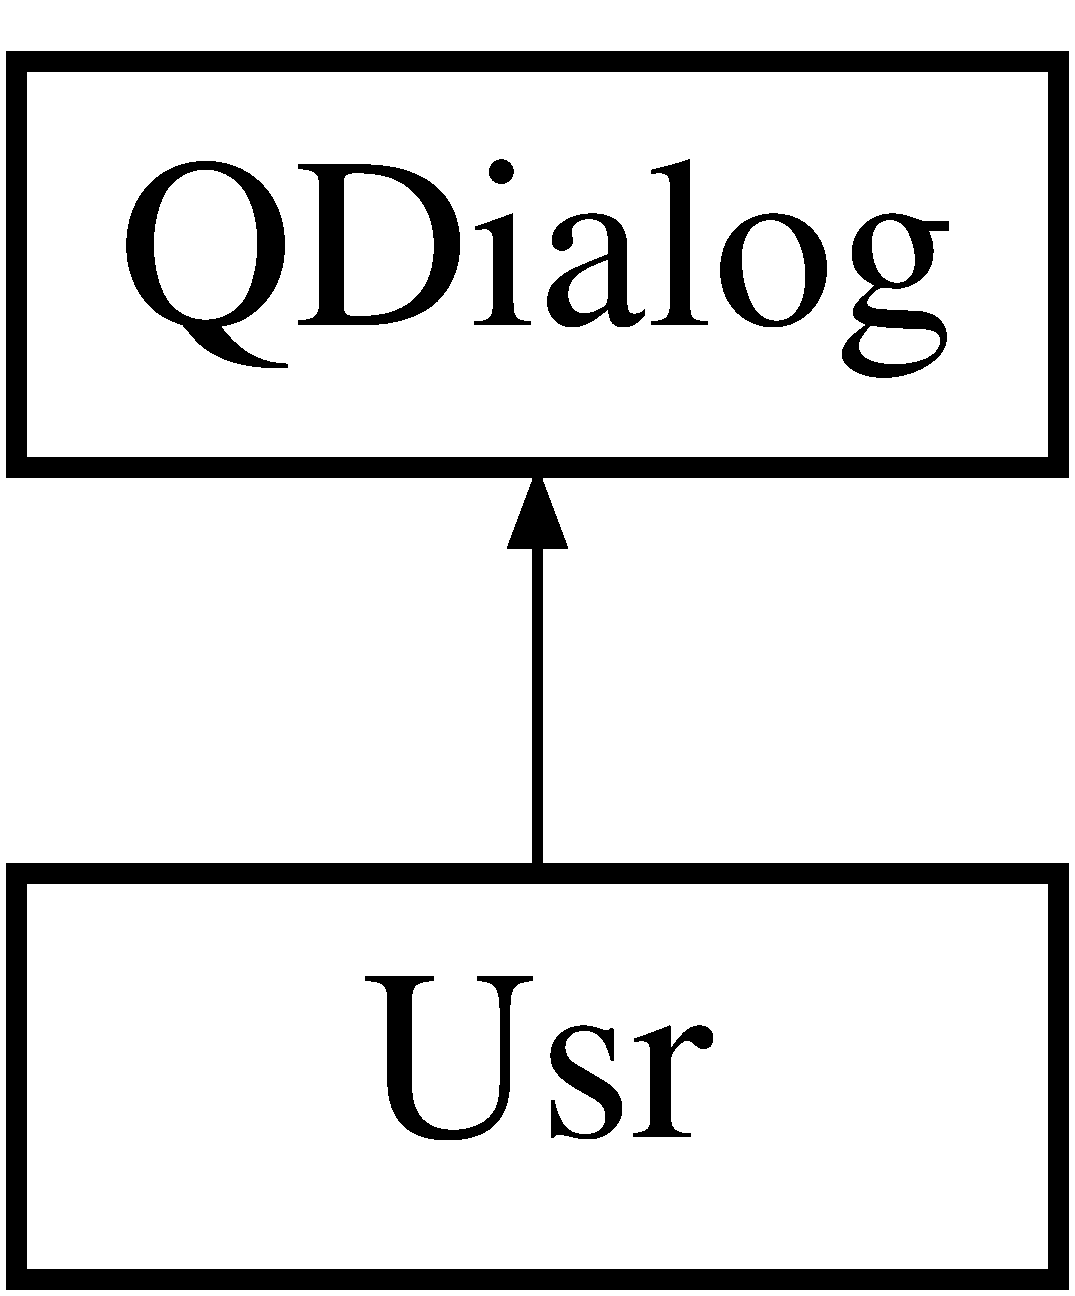
\includegraphics[height=2.000000cm]{class_usr}
\end{center}
\end{figure}
\subsection*{Public Member Functions}
\begin{DoxyCompactItemize}
\item 
\hyperlink{class_usr_a6bf567c68300ddd9a1825799b4a9803b}{Usr} (Q\+Widget $\ast$parent=0)
\begin{DoxyCompactList}\small\item\em \hyperlink{class_usr_a6bf567c68300ddd9a1825799b4a9803b}{Usr\+::\+Usr}. \end{DoxyCompactList}\item 
void \hyperlink{class_usr_a23ed125e9d15a4a2673a10280c106c74}{center\+Window} ()
\begin{DoxyCompactList}\small\item\em Writes the current foreground and background color of characters printed on the console into the argument color. \end{DoxyCompactList}\end{DoxyCompactItemize}


\subsection{Detailed Description}
Provide an example. 

This class is meant as an example. It is not useful by itself rather its usefulness is only a function of how much it helps the reader. It is in a sense defined by the person who reads it and otherwise does not exist in any real form.

\begin{DoxyNote}{Note}
Attempts at zen rarely work.
\end{DoxyNote}
\begin{DoxyAuthor}{Author}

\end{DoxyAuthor}
\begin{DoxyParagraph}{Author}
Camilla Lambrocco 
\end{DoxyParagraph}


\begin{DoxyVersion}{Version}

\end{DoxyVersion}
\begin{DoxyParagraph}{Revision}
1.\+1 
\end{DoxyParagraph}


\begin{DoxyDate}{Date}

\end{DoxyDate}
\begin{DoxyParagraph}{Date}
4/12/2015 
\end{DoxyParagraph}


\subsection{Constructor \& Destructor Documentation}
\hypertarget{class_usr_a6bf567c68300ddd9a1825799b4a9803b}{\index{Usr@{Usr}!Usr@{Usr}}
\index{Usr@{Usr}!Usr@{Usr}}
\subsubsection[{Usr}]{\setlength{\rightskip}{0pt plus 5cm}Usr\+::\+Usr (
\begin{DoxyParamCaption}
\item[{Q\+Widget $\ast$}]{parent = {\ttfamily 0}}
\end{DoxyParamCaption}
)\hspace{0.3cm}{\ttfamily [explicit]}}}\label{class_usr_a6bf567c68300ddd9a1825799b4a9803b}


\hyperlink{class_usr_a6bf567c68300ddd9a1825799b4a9803b}{Usr\+::\+Usr}. 


\begin{DoxyParams}{Parameters}
{\em parent} & \\
\hline
\end{DoxyParams}


\subsection{Member Function Documentation}
\hypertarget{class_usr_a23ed125e9d15a4a2673a10280c106c74}{\index{Usr@{Usr}!center\+Window@{center\+Window}}
\index{center\+Window@{center\+Window}!Usr@{Usr}}
\subsubsection[{center\+Window}]{\setlength{\rightskip}{0pt plus 5cm}void Usr\+::center\+Window (
\begin{DoxyParamCaption}
{}
\end{DoxyParamCaption}
)}}\label{class_usr_a23ed125e9d15a4a2673a10280c106c74}


Writes the current foreground and background color of characters printed on the console into the argument color. 

\begin{DoxyReturn}{Returns}
Void. 
\end{DoxyReturn}


The documentation for this class was generated from the following files\+:\begin{DoxyCompactItemize}
\item 
usr.\+h\item 
usr.\+cpp\end{DoxyCompactItemize}

%--- End generated contents ---

% Index
\newpage
\phantomsection
\addcontentsline{toc}{chapter}{Index}
\printindex

\end{document}
